\documentclass{article}
\usepackage{graphicx}
\graphicspath{ {./images/} }
\usepackage[section]{placeins}

\begin{document}

\begin{titlepage}
    \begin{center}
        \vspace*{1cm}
        
        \Huge
        \textbf{Fundamentals of Data Science}
        
        \vspace{0.5cm}
        \LARGE
        Freesound General-Purpuse Audio Tagging Challenge
        
        \vspace{1.5cm}
        
        \textbf{Lovro Bosnar}
        
        \vfill
        
        \Large
        Faculty of Physics and Applied Computer Science\\
        AGH University of Science and Technology\\
        Poland\\
        04.06.2018.
        
    \end{center}
\end{titlepage}

\tableofcontents
\newpage

\section{Introduction}
Project was selected among active competitions on Kaggle web site. Selected project is: Freesound 
General-Purpuse Audio Tagging Challenge. Core task is to automatically recognize sounds from a wide
range of real-word environments. \\
Because of large amount of different sounds, there is no reliable general-purpose audio tagging 
system existing. So, tagging is done manually.\\
Selected project is in category "Research".


\section{Task}
In this project challenge is to build a general-purpose automatic audio tagging system using a dataset 
of audio files covering a wide range of real-world environments. Dataset contains over 40 different 
labels (annotated using Google's AudioSet ontology). Some labels are not reliable. List of labels is in
figure \ref{fig:distrAudioSampl}.


\section{Dataset}
Dataset was developed by Freesound (MTG-UPF initiative) and Google Research’s Machine Perception Team.
Audio files for training were labelled ether manually or automatically. 3710 out of 9473 audio files are labelled
manually. Automatically labelled audio files may not be entirely reliable: 60-75 percent are estimated
to be correct.\\

\subsection{File descriptors}
Dataset of this project is following:
\begin{itemize}
 \item train.csv - file containing ground truth labels and indication of manual verification for 
  files in audio\_train directory
 \item audio\_train - directory containing audio (.wav) training files
 \item audio\_test - directory containing audio (.wav) test files
 \item sample\_submission.csv - file containing correct format of output for submission. 
  Contains file names from audio\_test directory.
\end{itemize}
Each row of train.csv file contains following columns:
\begin{itemize}
 \item fname - name of audio file (String)
 \item label - class for given audio file (String)
 \item manually\_verified - indication of manual verification of class (Boolean)
\end{itemize}

\subsection{Data analysis}
Complete dataset contains 18873 audio files. Labels are taken from Google's AudioSet Ontology.\\
All samples are provided as uncompressed PCM 16 bit, 44.1 kHz, mono audio files. Example is in  figure
\ref{fig:sampleBar}. Quality of sound can very much vary.\\
Reading and analysing audio files was done using $wave$ and $scipy.wavfile$ libraries.\\

\begin{figure}[!htb]
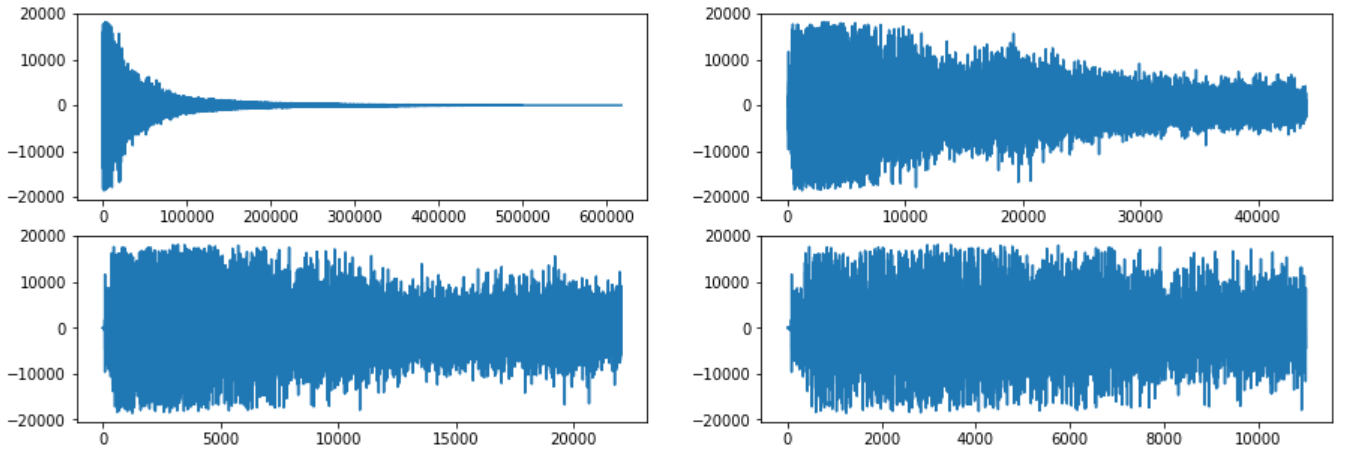
\includegraphics[width=15cm, height=5cm]{sampleBar}\\
\caption{Upper left: whole audio file. Upper right: 44100 samples. Lower left: 22050 samples. Lower right: 11025 samples}
\label{fig:sampleBar}
\centering
\end{figure}

Labels of sounds are unequally distributed in 41 classes.\\
Dataset is split into train and test.\\
For model training and system development \textbf{train set} is used. Train set contains 9473 samples unequally
distributed among 41 categories. Minimum number of samples per category is 94, maximum is 300. Duration
of samples ranges from 300ms to 30s. Number of manually verified audio files is 3710, rest are non-verified.
Use of non-verified audio samples is optional: estimated quality of 60-70 percent. Distribution of train
set by class is in figure \ref{fig:distrAudioSampl}.\\

\begin{figure}[!htb]
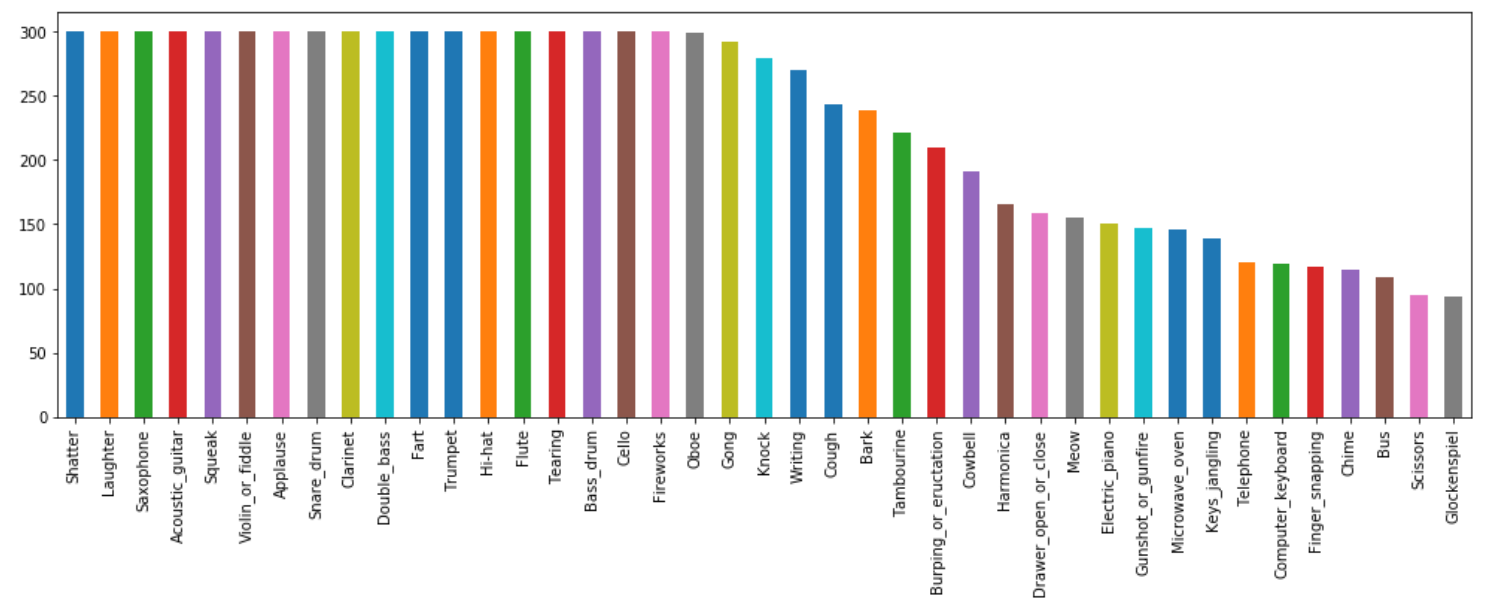
\includegraphics[width=15cm, height=7cm]{distrAudioSampl}\\
\caption{Distribution of all train audio samples by class}
\label{fig:distrAudioSampl}
\centering
\end{figure}

\textbf{Test set} is composed of 1600 samples with manually-verified annotations and with similar distribution as 
training set. Test set is complemented with 7800 padding sounds which are not used for scoring the system.\\
All samples in this dataset have single label.\\

\section{Feature extraction}
In this project chosen classification algorithms are: k nearest neighbours (kNN) and support vector machine (SVM).\\
Using raw audio files for these algorithms is not acceptable. But, future proposal would be using artificial neural network (ANN)
and deep learning which is able to classify directly from raw audio files as input.\\
Idea was to use spectrum of audio signal as starting point for modelling features. Spectrum of audio signal
is gain using Discrete Fourier Transform (DFT), because audio is discrete signal in time. Again using direct
result of DFT (FFT) is also not acceptable. So, Idea was to use spectrum in a way that would give useful 
information about signal. \\
Many approaches were proposed. Most widely used feature extraction from audio files is Mel-frequency cepstral 
coefficients (MFCC). This is state-of-art method therefore is used in this project.\\
Extraction of MFC coefficients is done using $librosa$ library. Proposal for future work be extracting additional 
information using this library.

\subsection{MFCC}
Method is introduced by Davis and Mermelstein in the 1980's. Before MFCC, used methods were Linear Prediction 
Coefficients (LPC) and Linear Prediction Cepstral Coefficients (LPCC). But, MFCC is state-of-the-art ever since.\\
First we will see basic steps of extracting MFC coefficients. Then we will try to further model features using MFCCs.
Also, additional very useful features called delta and delta delta will be introduced. delta and delta delta are 
calculated from MFCC and represent useful information about audio data.\\

\subsubsection{How MFCC works?}
It is important to know basics of this method because we can then use result for further modelling.\\
Firstly, audio signal is divided in stationary overlapping segments of 20-40 ms length. Segments are called frames.
Every frame is simple enough to be described with not too much spectral coefficients.\\
It is important to note that all other steps are made for every frame. So, MFCC result will matrix, and one of 
dimension is number of frames.\\
In second step, window function is applied to frame. Reason for this is avoiding spectral leakage introduced by
splitting audio in frames.\\
In third step, DFT is applied to frame. Result is spectrum, in other words vector of k elements. Every element 
represents spectral coefficient. Using spectrum estimation of power spectrum is calculated - periodogram. DFT is 
done for 512 points, we take 257.\\
In forth step, power spectrum is grouped using Mel-spaced filterbanks. This is a set of 20-40 triangular filters.
Usually 26 is used. Mel-spaced means that triangular filters are narrow at low frequencies and wide at high 
frequencies. Mel-spacing is inspired by human hearing system. Result of this step is vector of 26 elements that
represent grouped power spectrum.\\
In final step we calculate cepstrum coefficients. By definition cepstrum is result inverse DFT of log power spectrum.
So, log power spectrum is calculated. But instead of inverse DFT, Discrete Cosine Transformation (DCT) is made. 
Reason for DCT is breaking correlation between frames (note that frames are overlapping and thus are correlated).
Result is vector of 26 elements. Usually 12 are taken. Higher frequencies bring more negative than positive effect
as features.\\
In this project we will take $n=12$ MFC coefficients per frame. Number of frames is $m$, later will be explained how 
many are there for this specific problem. So MFCC matrix will have dimensions $[n x m]$. Result for one audio 
file is in figure \ref{fig:mdda}. \\

\begin{figure}[!htb]
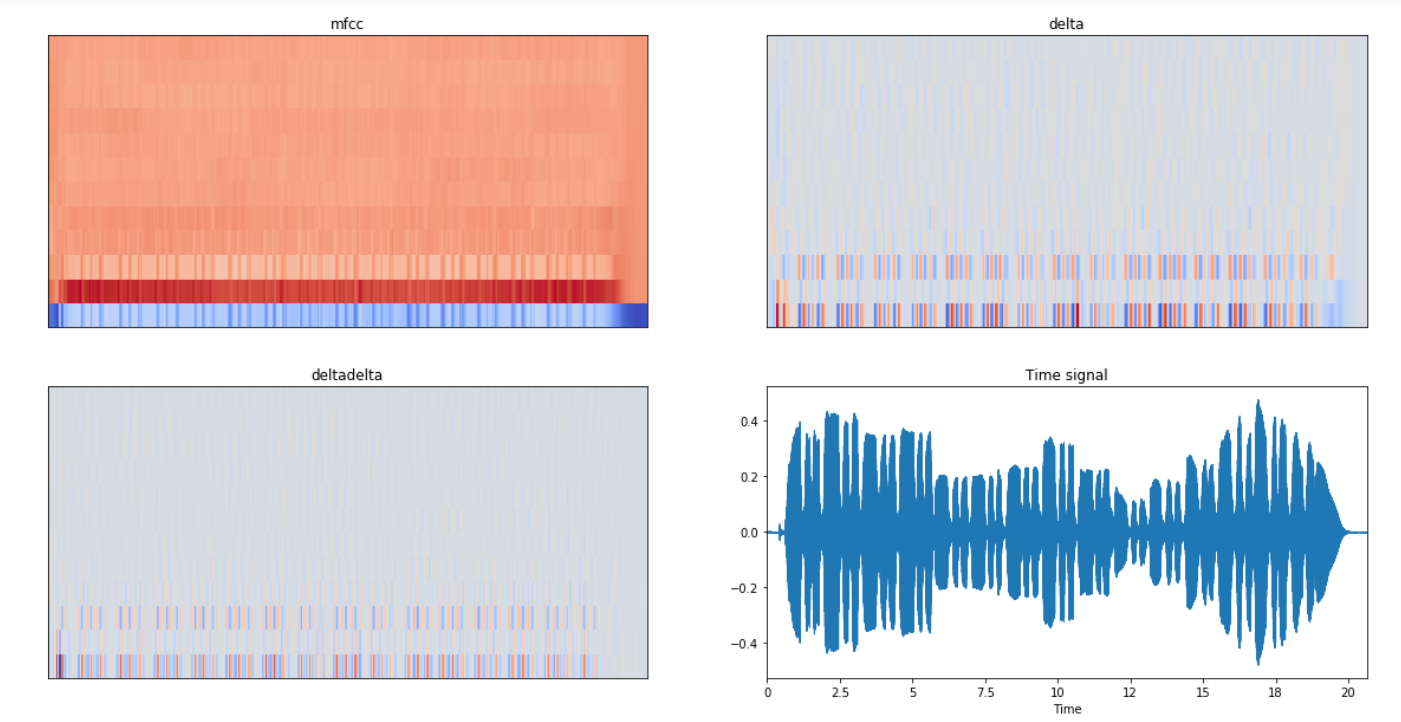
\includegraphics[width=15cm, height=7cm]{mdda}\\
\caption{Upper Left: MFCC. Upper right: delta. Lower left: delta delta. Lower right: audio file in time.}
\label{fig:mdda}
\centering
\end{figure}


\subsubsection{Delta and delta delta}
Next to MFC coefficients very useful information is Delta and Delta Delta. These coefficients carry information about
dynamics over time.\\
Delta is local estimate of the derivative of first order.\\
Delta Delta local is estimate of the derivative of second order.\\
Both Delta and Delta Delta matrices have same dimensions as MFCC matrix. Example is in figure \ref{fig:mdda}.\\

\subsection{Use of MFC coefficients}
Audio files are different lengths. So, MFCC, Delta and Delta Delta matrices for every file will have different dimensions. 
That is not acceptable input for classifier.\\
In following section we will discuss ways to solve this problem.\\

\subsubsection{Using original MFC coefficients}
One approach is to use original MFCCs. So first we need to find longest file in order to find maximum number of audio 
samples. Then it is needed to preform padding with zeros so every file will have same length.\\
Idea for future work would be removing zeros from start and end of audio files. In that way result will be smaller 
arrays. It is not done in this project because this method requires careful consideration (e.g. what if zeros are inside of 
audio file?)\\
After analysis we can see that longest file has 1323000 samples. Distribution of number of samples per audio
files is given in figure \ref{fig:distrSamplAudio}. So, we need to add zeros to every file that has smaller amount
of samples. Example of file before adding zeros is in figure \ref{fig:mdda}, and same file after adding zeros is in figure 
\ref{fig:mddazeros}. Question for further work is should be zeros be added to start or end of audio file and which is better? Also random
offset could be taken. In this project zeros were added on the end of audio file. \\
After analysis for file that has $m=1323000$ samples and $n=12$ MFCC per frame resulting MFCC matrix will have dimensions [12 x 2584]. \\
Problem with this approach is huge amount of information just for one audio file. But this is starting point for other methods.
If we take in account all audio files ($N$) result of this step will be matrix [N x 12 * 2584] where MFCC matrix for every
file is flatten from [12 x 2584] to array of 12 * 2584 elements. Same dimensions will have resulting delta and delta delta matrices.\\

\begin{figure}[!htb]
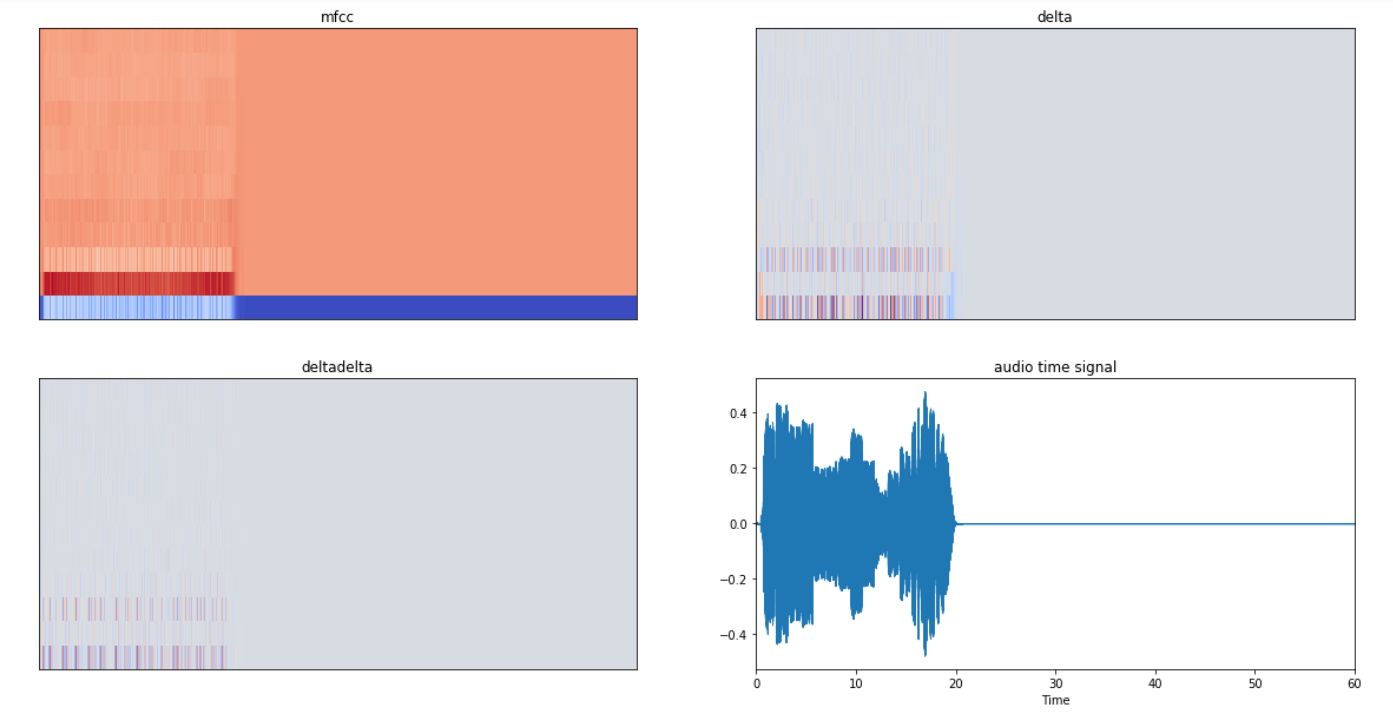
\includegraphics[width=15cm, height=7cm]{mddazeros}\\
\caption{Upper Left: MFCC. Upper right: delta. Lower left: delta delta. Lower right: audio file in time.}
\label{fig:mddazeros}
\centering
\end{figure}

\begin{figure}[!htb]
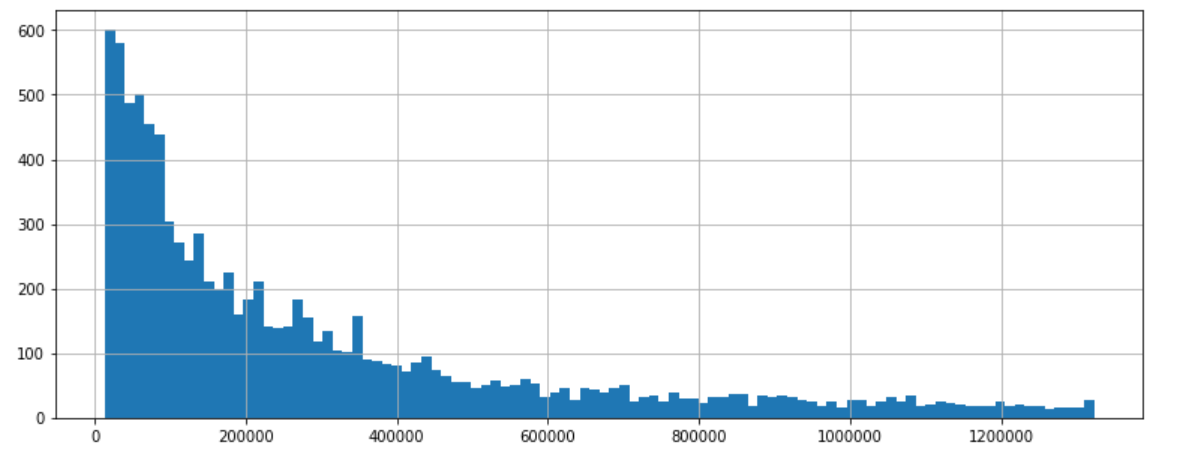
\includegraphics[width=10cm, height=4cm]{noOfSamples}\\
\caption{Number of samples for every audio file.}
\label{fig:distrSamplAudio}
\centering
\end{figure}


\subsubsection{Creating new features using PCA}
For one audio file we have $m$ frames, and every frame has vector of $n$ MFCCs, $n$ Delta and $n$ Delta Delta. So, one 
audio file is represented by three matrices dimensions [$n$ x $m$]. Idea is to use principal component analysis (PCA) to 
reduce each matrix into vector of $n*5$ elements. This is flattened vector from resulting matrix of PCA method with reduction 
to 5 dimensions.\\
We have N audio files. So, for every audio file resulting matrices will have dimension [N x n*5]. If we take real numbers 
in case then N = 9473 and n = 12. Also, we can just take manually verified audio files, then N = 3710.\\
Problem with this approach is too large reduction of dimensions, and loss of data. Because PCA was used to reduce dimensions
from $m=2584$ to $m=5$.
Proposal for future work would be using PCA for reduction to higher dimensions than 2 and assessing quality. \\
Firstly, problem is large amount of data so time and memory complexity is high so sampling data would be solution. Second problem
is relatively large amount of data even after reduction.\\

\subsubsection{Creating new features using statistical moments}
Another approach is to calculate average, standard deviation, minimal value, maximal value and skewness for mfcc,
delta and delta delta matrices by rows for every file. So, every file will have 5 vectors for MFCC, Delta and Delta Delta. 
In total 15 vectors per file. Every vector will have length $n=12$.\\
Problem with this approach is potentially loss of data. With current domain knowledge it is hard to deduce if this method of
creating new features is containing enough information for classifiers.\\
Proposal for future work would be analysis of quality using this features accompanied with better domain knowledge.\\


\section{Algorithms}
As mentioned for this project is used K nearest neighbours (kNN) and support vector machine (SVM). \\
Other classifiers that were also proposed: Artificial neural networks (ANN) and deep learning methods, 
Gaussian mixture model (GMM). Also, combination of classifiers with Hidden Markov Models (HMM) was proposed. 
This is just a hint for future work on this project and It will not be considered in this paper.\\
It is important to point out that because of large amount of train data and large time and memory complexity 
for feature extraction we sampled 3000 out of 3700 manually verified train data for training which consist of 9473
examples. It is important to note that manually verified set is good representation of whole dataset. We can see that 
comparing figures \ref{fig:distrAudioSampl} and \ref{fig:distrAudioSamplMan}
For evaluation we used 5 fold cross validation.\\

\begin{figure}[!htb]
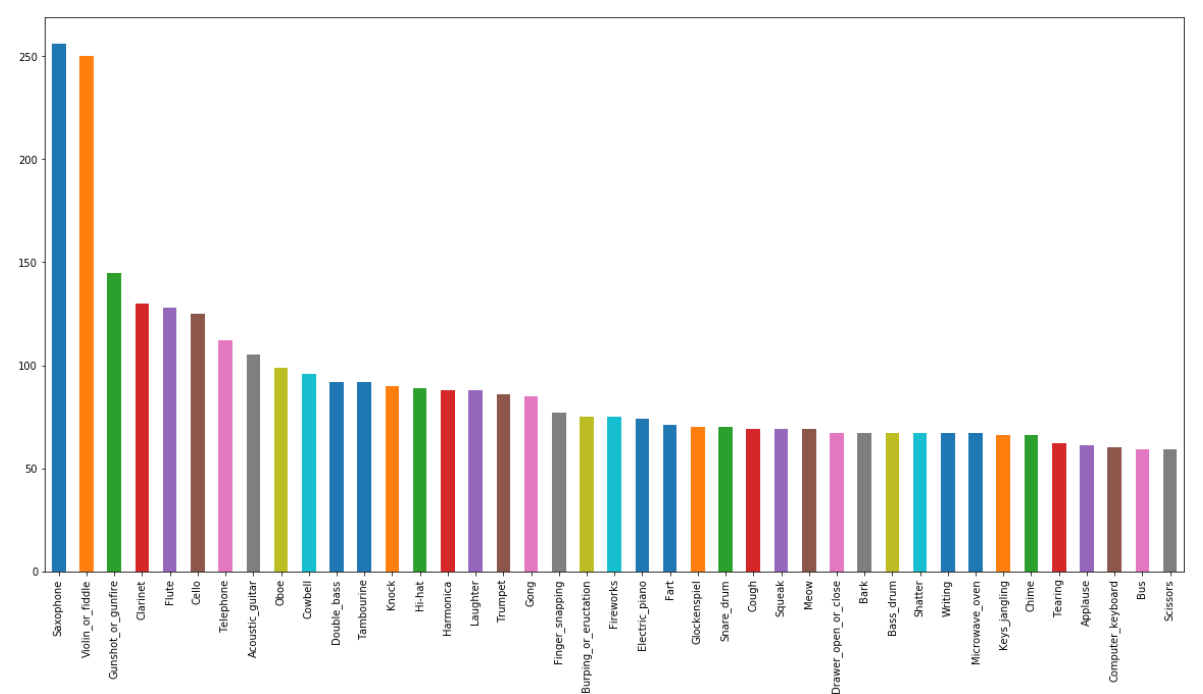
\includegraphics[width=15cm, height=7cm]{distrAudioSamplMan}\\
\caption{Distribution of manually verified train audio samples by class}
\label{fig:distrAudioSamplMan}
\centering
\end{figure}

\subsection{kNN}
This algorithm was chosen because of simplicity, popularity and finally comparison with more complex models like
SVM.\\
Used library is $sklearn.neighbors.KNeighborsClassifier$. \\

\subsubsection{About KNN}
New examples are classified depending on k nearest neighbours. So, class of new example is depending on class 
majority of nearest neighbours. \\
Number of nearest neighbours - k is given by user. Also, important parameter is choice of metric for calculating
distances to other examples. \\

\subsubsection{Training and validation}
Next to feature extraction it is necessary to choose best hyper parameters: number of nearest neighbours and metric
for calculating distances.\\
First we are using train set where features were modelled with PCA.\\
Nearest neighbours were chosen from set: {1, 4, 8, 16, 20}. Results are in figure \ref{fig:knnNN1}.\\

\begin{figure}[!htb]
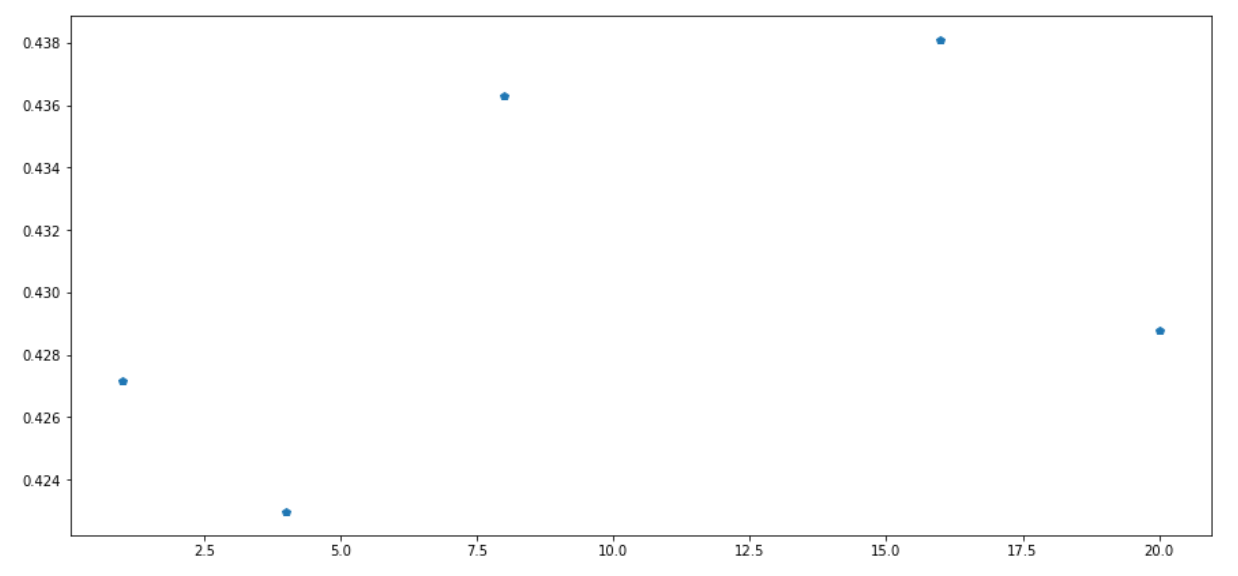
\includegraphics[width=12cm, height=5cm]{knnNN1}\\
\caption{Accuracy for different number of nearest neighbours.}
\label{fig:knnNN1}
\centering
\end{figure}


Metrics were chosen from set: {'cosine', 'manhattan', 'minkowski', 'euclidean', 'chebyshev'}. Results are in figure \ref{fig:knnmet1}.\\

\begin{figure}[!htb]
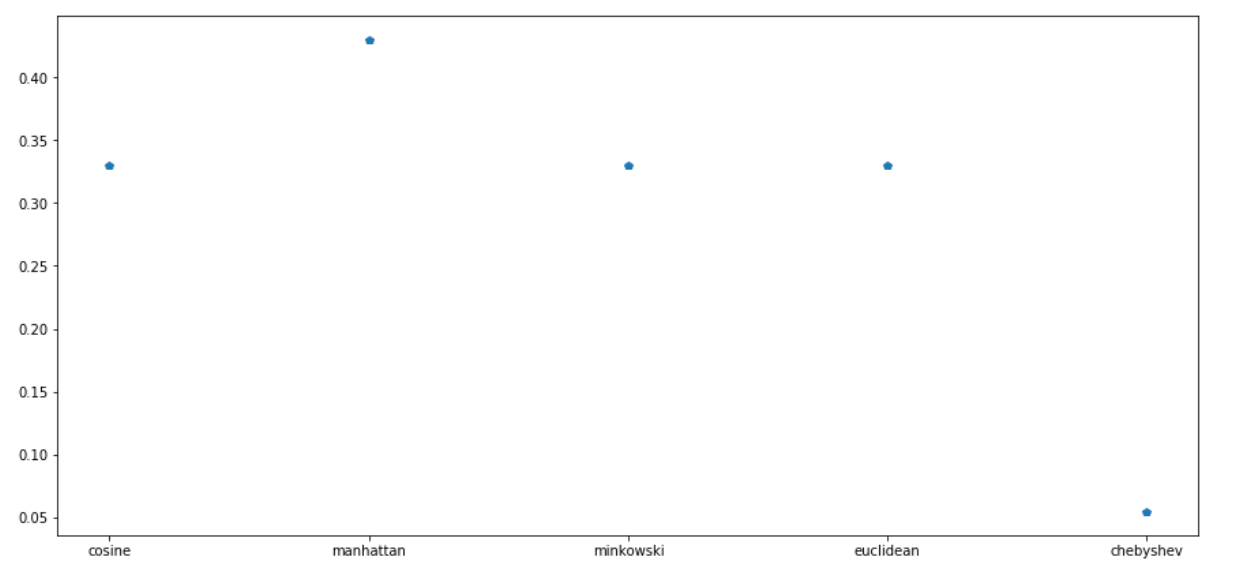
\includegraphics[width=12cm, height=5cm]{knnMet1}\\
\caption{Accuracy for different metrics.}
\label{fig:knnmet1}
\centering
\end{figure}

Best accuracy for given nearest neighbours and metrics for this training data is 43\% which is worse than random classifier.\\

Next we are using train set where features were modelled with statistical moments.\\

Nearest neighbours were chosen from set: {1, 4, 8, 16, 20}. Results are in figure \ref{fig:knnNN2}.\\

\begin{figure}[!htb]
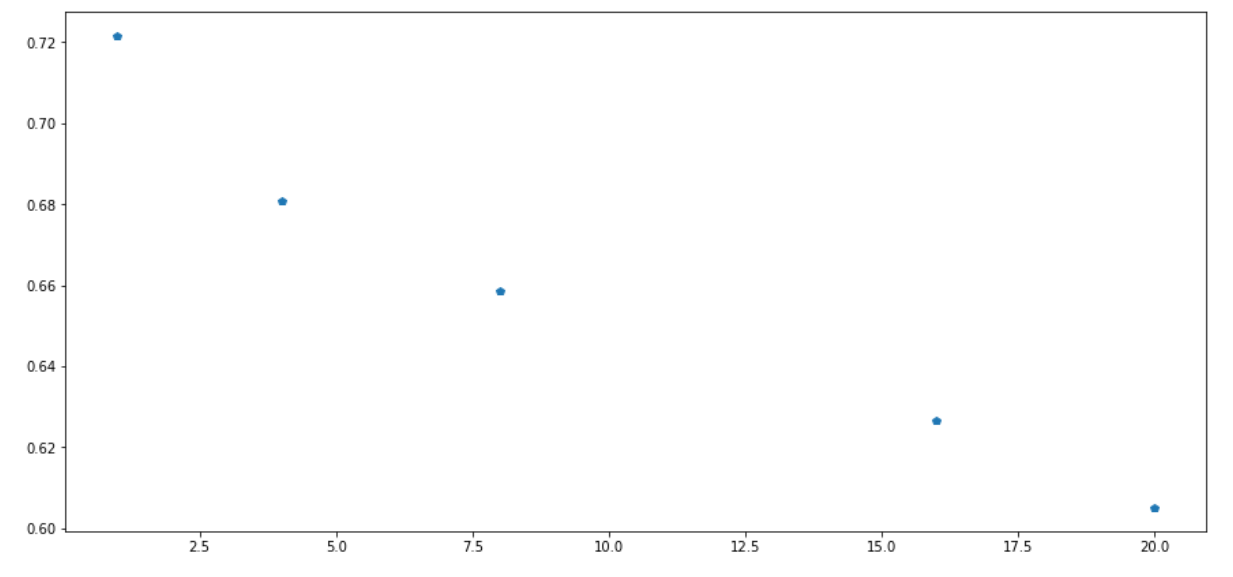
\includegraphics[width=12cm, height=5cm]{knnNN2}\\
\caption{Accuracy for different number of nearest neighbours.}
\label{fig:knnNN2}
\centering
\end{figure}


Metrics were chosen from set: {'cosine', 'manhattan', 'minkowski', 'euclidean', 'chebyshev'}. Results are in figure \ref{fig:knnmet2}.\\

\begin{figure}[!htb]
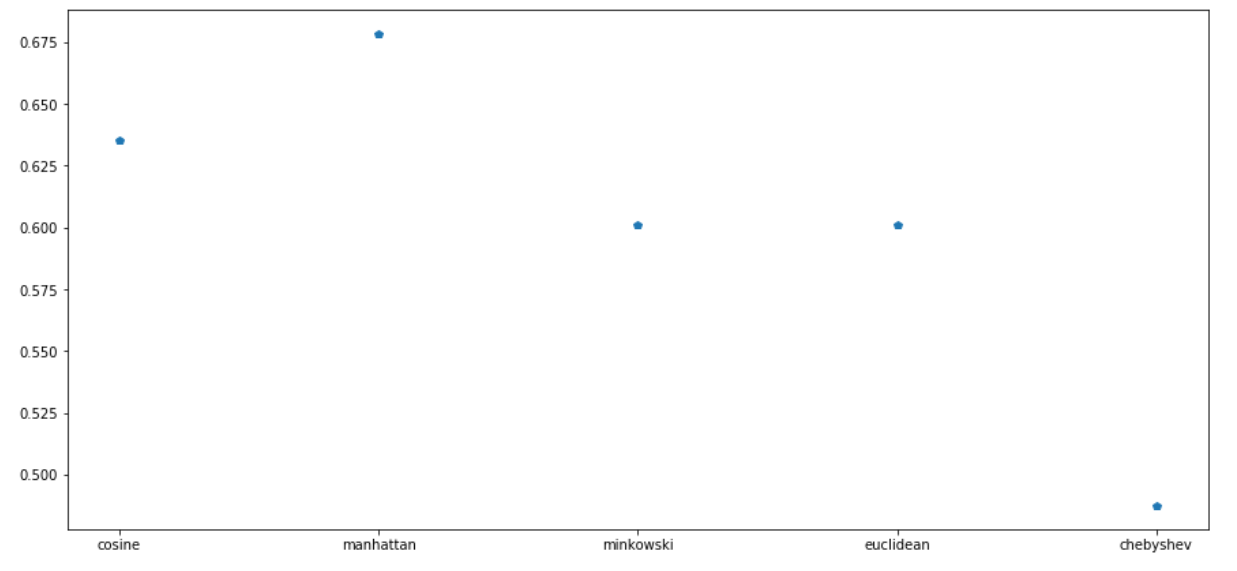
\includegraphics[width=12cm, height=5cm]{knnMet2}\\
\caption{Accuracy for different metrics.}
\label{fig:knnmet2}
\centering
\end{figure}

Accuracy is highest for k = 1. We will chose k = 3 because of hope of better generalization for test set.\\
Accuracy for k = 3 and metric = 'manhattan' and this training data is 69\% which is better than random classifier. 
For both datasets we can see that metric is the same. But, interestingly enough, number of nearest neighbours which
scores best result for first data is 16! 
So, we use number of nearest neighbours: 3, best metric is 'manhattan' and better train set is one modelled with statistical
moments. This parameters are used to classify given Kaggle test set.\\

\subsubsection{Discussion}
We can see that kNN preforms best with k = 3 and metric 'manhattan', training set with features modelled with statistical moments was used. Averaged 5 fold cross validation for this gave around 69\% accuracy which is better then random classifier. \\
Explanation for poor result is the way of using MFCC, delta and delta delta features. As PCA has reduced dimensionality
drastically so lots of information was lost. It is crucial to find to what dimension to reduce the dataset. \\
As for other train set (with statistical moments), poor results could be because of lost information and not using additional
information that could compensate this loss.\\
Certainly, if we used more than 3000 train examples results would be better.\\
Additionally poor result could be explained because of kNN which is not recommended classifier to be used, at least not used alone.\\
Submission of classified test set on Kaggle resulted in 0.617 accuracy (figure \ref{fig:kaggle}.)\\

\begin{figure}[!htb]
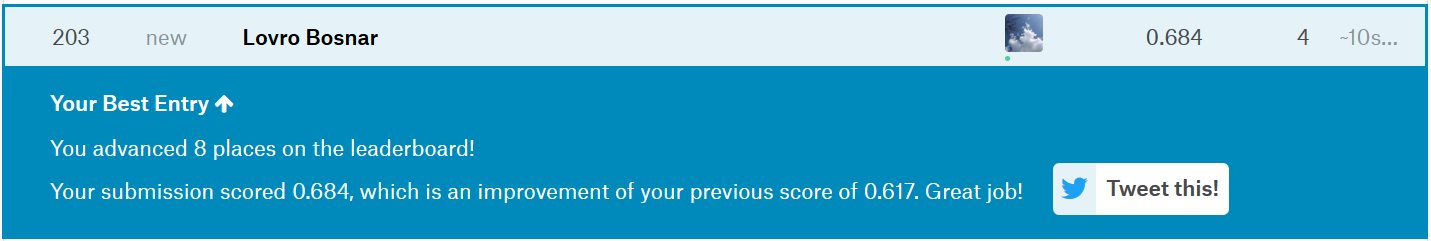
\includegraphics[width=15cm, height=3cm]{kaggle}\\
\caption{Kaggle result for kNN. Previous result: kNN. Best result: SVM}
\label{fig:kaggle}
\centering
\end{figure}


\subsection{SVM}
Support vector machine (SVM) is very powerful classifier. It is recommended to be used in audio classification. Many 
approaches are not using SVM alone, but with other models as well. In this project we will use SVM alone.\\
Used library is $sklearn.svm.SVC$.\\

\subsubsection{About SVM}
SVM classification is based on support vectors which are training examples. Idea is to form margin between classes. Margin 
is an area between classes which is bounded by hyperplane. Hyperplane is "supported" by examples from classes and it should 
be maximised. So, SVM is linear model.\\
In basic version, SVM is not allowing examples to be inside of margin. This version couldn't separate linearly inseparable 
examples. This version is called maximal margin classifier.\\
Then kernel trick is used which is transforming data from linearly inseparable data in higher dimension to become linearly
separable. With kernel trick maximal margin classifier is able to classify initial linearly inseparable examples. It is important
to note that kernel decision is crucial for performance, for some kernels (e.g. RBF) additional parameter $gamma$ is used.
$gamma$ is regulating influence of example.\\
In another version SVM is allowing examples to be inside of margin. This version is called soft margin classifier. In this 
version crucial parameter is penalty parameter $C$ which is regulating acceptable amount of examples in margin.\\
Most advanced version is soft margin SVM with kernel trick. In this approach parameters: penalty $C$, kernel, degree of polynomial 
(if used as kernel), $gamma$ should be used carefully to obtain best possible results.\\

\subsubsection{Training and validation}
As explained optimal parameters are important for best results. \\
Firstly, chosen parameters are $C = 1$, $gamma = 1$, kernel: RBF.\\
For dataset modelled with PCA, average result of 5 fold CV is 0.0713530256396.\\
For dataset modelled with statistical moments, average result of 5 fold CV is 0.0713530256396.\\

Next,chosen parameters are $C = 1$, $gamma = 1$, kernel: polynomial, with degree 5.\\
For dataset modelled with PCA, average result of 5 fold CV is 0.727506782017.\\
For dataset modelled with statistical moments, average result of 5 fold CV is 0.106049306854.\\

From this results we can see that RBF kernel is not good choice. Better choice is polynomial kernel. Again,
features modelled with statistical moments are resulting in much better results.\\

\subsubsection{Discussion}
Explanation for this results, firstly, would be choice of hyper-parameters. SVM is very sensitive to chosen penalty $C$, kernel
function and $gamma$. To obtain better results exhaustive grid search along this parameters is needed. Because
of large amount of training data parameters were chosen manually. Proposal for future work would be sampling data and using 
grid search for best parameters.\\
Also, when polynomial kernel is used optimal degree should be chosen, so search for best degree is also needed.\\
Next, whole training set was not used. With more examples, model would generalise better.\\
Furthermore, because of lack of domain knowledge the way of modelling features is not optimal and lots of information
was lost.\\
Submission of classified test set on Kaggle resulted in 0.684 accuracy. Figure \ref{fig:kaggle}.


\section{Summary}
In this project general purpose audio tagging system was built. For input we were given ~9400 audio examples for train and
another ~9400 audio examples for test. As mentioned whole dataset was not used so idea for future work would be using more data
or sample data with different technique. Also, finding correctly labelled examples among non-manually labelled dataset would be
another challenge.\\
Features were modelled using MFC coefficients. Large amount of information of MFCCs was additionally processed with PCA and
statistical moments. We have seen that for PCA method optimal dimensions should be found. Also better domain knowledge should be 
acquired in order to model fratures better.\\
We used kNN and SVM classifiers. For both algorithms, beside optimal features, we needed to chose optimal parameters. In case
of SVM exhaustive grid search should be preformed.\\
Results on kaggle test set was 0.617 for kNN and 0.684 for SVM accurate. Explanation of results is the way of modelling 
features, not using whole data set and not using optimal parameters.\\ 

\begin{thebibliography}{9}
 \bibitem{a} Beginner guide to Audio data: $https://www.kaggle.com/fizzbuzz/beginner-s-guide-to-audio-data$
 \bibitem{b} XGB using MFCC and opanichev's features: $https://www.kaggle.com/amlanpraharaj/xgb-using-mfcc-opanichev-s-features-lb-0-811$
 \bibitem{c} k-nearest neighbors algorithm: $https://en.wikipedia.org/wiki/K-nearest_neighbors_algorithm$
 \bibitem{d} SVM understanding math: $https://www.svm-tutorial.com/2014/11/svm-understanding-math-part-1/$
 \bibitem{e} Understanding MFCC: $practicalcryptography.com/miscellaneous/machine-learning/guide-mel-frequency-cepstral-coefficients-mfccs/$
\end{thebibliography}



\end{document}